\documentclass{standalone}
\usepackage{tikz}
\usetikzlibrary{calc,fadings,decorations.pathreplacing}
\usepackage{verbatim}
\usepackage{xparse}
%% helper macros
\newcommand\pgfmathsinandcos[3]{%
  \pgfmathsetmacro#1{sin(#3)}%
  \pgfmathsetmacro#2{cos(#3)}%
}
\newcommand\LongitudePlane[3][current plane]{%
  \pgfmathsinandcos\sinEl\cosEl{#2} % elevation
  \pgfmathsinandcos\sint\cost{#3} % azimuth
  \tikzset{#1/.style={cm={\cost,\sint*\sinEl,0,\cosEl,(0,0)}}}
}
\newcommand\LatitudePlane[3][current plane]{%
  \pgfmathsinandcos\sinEl\cosEl{#2} % elevation
  \pgfmathsinandcos\sint\cost{#3} % latitude
  \pgfmathsetmacro\yshift{\cosEl*\sint}
  \tikzset{#1/.style={cm={\cost,0,0,\cost*\sinEl,(0,\yshift)}}} %
}
\newcommand\DrawLongitudeCircle[2][1]{
  \LongitudePlane{\angEl}{#2}
  \tikzset{current plane/.prefix style={scale=#1}}
   % angle of "visibility"
  \pgfmathsetmacro\angVis{atan(sin(#2)*cos(\angEl)/sin(\angEl))} %
  \draw[current plane] (\angVis:1) arc (\angVis:\angVis+180:1);
  \draw[current plane,dashed] (\angVis-180:1) arc (\angVis-180:\angVis:1);
}
\newcommand\DrawLatitudeCircle[2][2]{
  \LatitudePlane{\angEl}{#2}
  \tikzset{current plane/.prefix style={scale=#1}}
  \pgfmathsetmacro\sinVis{sin(#2)/cos(#2)*sin(\angEl)/cos(\angEl)}
  % angle of "visibility"
  \pgfmathsetmacro\angVis{asin(min(1,max(\sinVis,-1)))}
  \draw[current plane] (\angVis:1) arc (\angVis:-\angVis-180:1);
  \draw[current plane,dashed] (180-\angVis:1) arc (180-\angVis:\angVis:1);
}

%% document-wide tikz options and styles

\tikzset{%
  >=latex, % option for nice arrows
  inner sep=0pt,%
  outer sep=2pt,%
  mark coordinate/.style={inner sep=0pt,outer sep=0pt,minimum size=4pt,
  fill=black,circle}%
}

\begin{document}
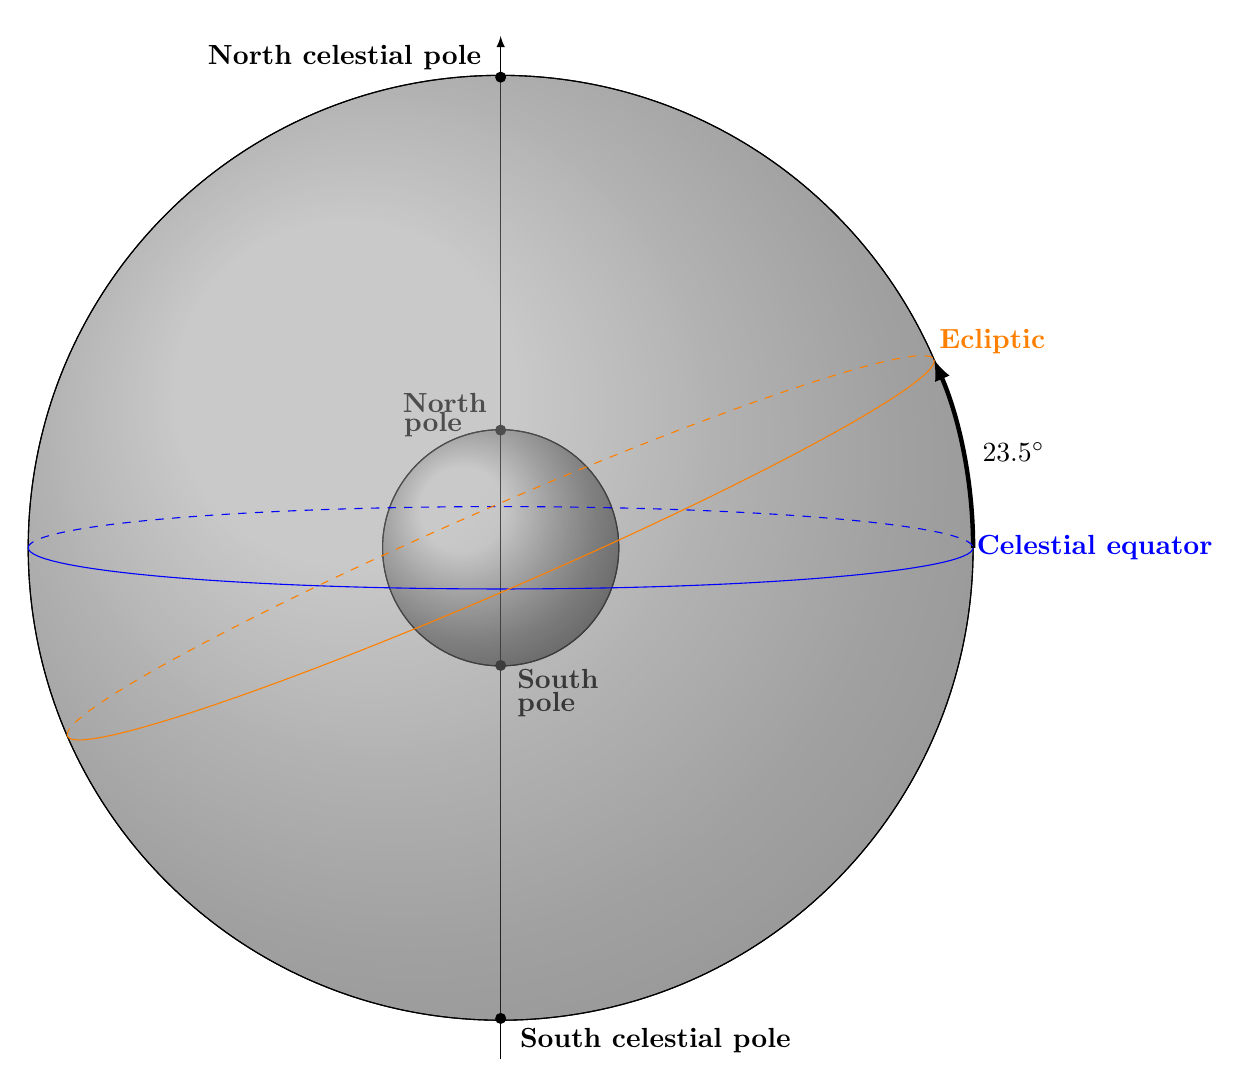
\begin{tikzpicture} % "THE GLOBE" showcase


    \def\R{1.5} % sphere radius
    \def\angEl{5} % elevation angle
    \def\angAz{105} % azimuth angle
    \def\angPhi{-40} % longitude of point P
    \def\angBeta{19} % latitude of point P

    \pgfmathsetmacro\H{\R*cos(\angEl)} % distance to north pole
    \tikzset{xyplane/.style={cm={cos(\angAz),sin(\angAz)*sin(\angEl),-sin(\angAz),
                                  cos(\angAz)*sin(\angEl),(0,-\H)}}}
    \LongitudePlane[xzplane]{\angEl}{\angAz}
    \LatitudePlane[equator]{\angEl}{0}

     \filldraw[ball color=white, fill opacity=1] (0,0) circle (\R);
    \draw (0,0) circle (\R);
    \coordinate (O) at (0,0);
    \coordinate[mark coordinate] (N) at (0,\H);
    \coordinate[mark coordinate] (S) at (0,-\H);
%		\coordinate (horizon) at (-30.0:\R);
%		\coordinate (equator) at (\H,0);


    \draw[->] (0,-\H-5) -- (0,\R+5) node[above] {}; %axis of rotation
%		\draw[->,rotate=-30.0] (0,-\H-5) -- (0,\R+5) node[above] {\bf{Zenith}}; %axis of rotation

    \path[xzplane] (\R,0) coordinate (XE);

%		\DrawLatitudeCircle[\R,color=blue]{0} % equator
%		\DrawLatitudeCircle[\R,rotate=23.5,color=red]{0}
%		\node[right,color=red] at (horizon) {\bf{Horizon}};
%		\node[above=9pt, right=-5pt, color=blue] at (equator) {\bf{Equator}};
%		\node[label={above right:\bf{Equator}}] at (equator) {};

    \node[above=10pt, left=3pt] at (N) {\bf{North}};
    \node[above=2pt, left=12pt] at (N) {\bf{pole}};

    \node[below=5pt, right=4pt] at (S) {\bf{South}};
    \node[below=14pt, right=4pt] at (S) {\bf{pole}};

    \def\R{6} % sphere radius
    \def\angEl{5} % elevation angle
    \def\angAz{105} % azimuth angle
    \def\angPhi{-40} % longitude of point P
    \def\angBeta{19} % latitude of point P

    \pgfmathsetmacro\H{\R*cos(\angEl)} % distance to north pole
    \tikzset{xyplane/.style={cm={cos(\angAz),sin(\angAz)*sin(\angEl),-sin(\angAz),
                                  cos(\angAz)*sin(\angEl),(0,-\H)}}}
    \LongitudePlane[xzplane]{\angEl}{\angAz}
    \LatitudePlane[equator]{\angEl}{0}

    \filldraw[ball color=white, fill opacity=0.3] (0,0) circle (\R);
    \draw (0,0) circle (\R);

    \coordinate (O) at (0,0);
    \coordinate[mark coordinate] (N) at (0,\H);
    \coordinate[mark coordinate] (S) at (0,-\H);
		\coordinate (Equator) at (\H,0);
		\coordinate (Ecliptic) at (23.5:\R);
    \path[xzplane] (\R,0) coordinate (XE);

		\draw[->,ultra thick] (0:\R) arc (0:23.5:\R);
		\coordinate (tilt) at (11.75:\R);
		\node[right=5pt] at (tilt) {$23.5^{\circ}$};
%		\coordinate (obslat) at (75:0.4*\R);
%		\node[above=5pt] at (obslat) {$30^{\circ}$};
		\DrawLatitudeCircle[\R,color=blue]{0} % equator
%		\draw 
		\DrawLatitudeCircle[\R,rotate=23.5, color=orange]{0} % ecliptic
		\node[right, color=blue] at (Equator) {\textbf{Celestial equator}};
		\node[above right, color=orange] at (Ecliptic) {\textbf{Ecliptic}};
%		\node[label={above right:\bf{Celestial horizon}},color=red] at (Horizon) {};
%		\node[label={right:\bf{Celestial equator}},color=red] at (Equator) {};

%		\DrawLongitudeCircle[\R]{\angAz+15}{} % xzplane

    \node[above=7pt, left=5pt] at (N) {\bf{North celestial pole}};
    \node[below=8pt, right=5pt] at (S) {\bf{South celestial pole}};

\end{tikzpicture}
\end{document} 
